\documentclass{standalone}
\usepackage{tikz}
\usetikzlibrary{patterns, positioning}
\usepackage[sfdefault]{ClearSans} %% option 'sfdefault' activates Clear Sans as the default text font
\usepackage[T1]{fontenc}

\begin{document}
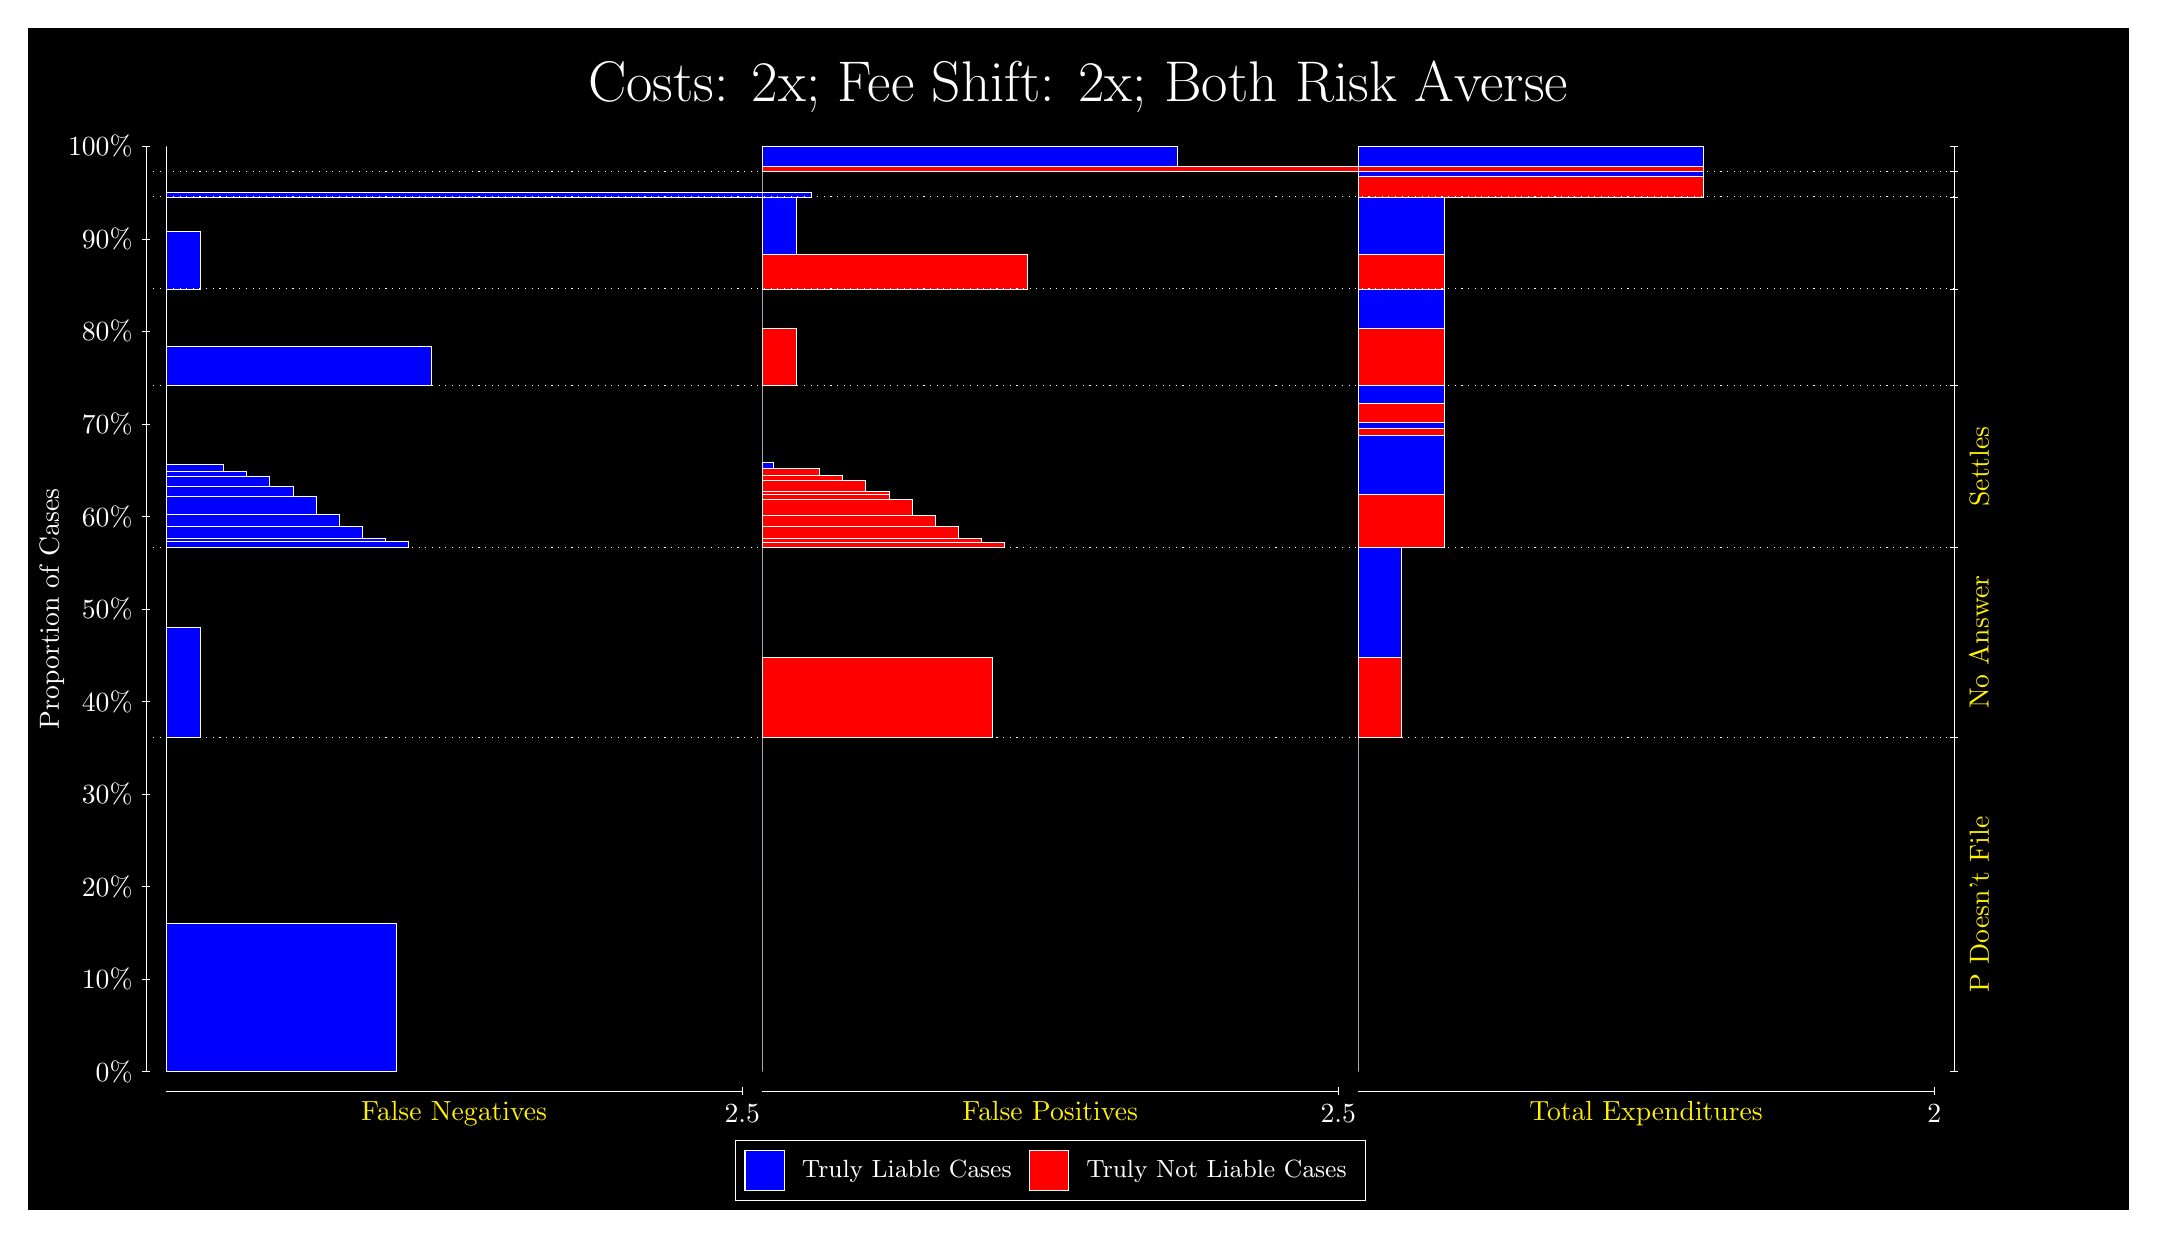
\begin{tikzpicture}
\draw[fill=black] (0,0) rectangle (26.667,15);
\draw[text=white] (0,13.5) rectangle (26.667,15) node[midway] {\huge Costs: 2x; Fee Shift: 2x; Both Risk Averse};
\draw[white, very thin] (1.5,1.75) -- (1.5,13.5);
\node[rotate=90, text=white, anchor=center] at (0.3, 7.625) {Proportion of Cases};
\draw[white, very thin] (1.45,1.75) -- (1.55,1.75);
\node[text=white, anchor=east] at (1.45, 1.75) {0\%};
\draw[white, very thin] (1.45,2.925) -- (1.55,2.925);
\node[text=white, anchor=east] at (1.45, 2.925) {10\%};
\draw[white, very thin] (1.45,4.1) -- (1.55,4.1);
\node[text=white, anchor=east] at (1.45, 4.1) {20\%};
\draw[white, very thin] (1.45,5.275) -- (1.55,5.275);
\node[text=white, anchor=east] at (1.45, 5.275) {30\%};
\draw[white, very thin] (1.45,6.45) -- (1.55,6.45);
\node[text=white, anchor=east] at (1.45, 6.45) {40\%};
\draw[white, very thin] (1.45,7.625) -- (1.55,7.625);
\node[text=white, anchor=east] at (1.45, 7.625) {50\%};
\draw[white, very thin] (1.45,8.8) -- (1.55,8.8);
\node[text=white, anchor=east] at (1.45, 8.8) {60\%};
\draw[white, very thin] (1.45,9.975) -- (1.55,9.975);
\node[text=white, anchor=east] at (1.45, 9.975) {70\%};
\draw[white, very thin] (1.45,11.15) -- (1.55,11.15);
\node[text=white, anchor=east] at (1.45, 11.15) {80\%};
\draw[white, very thin] (1.45,12.325) -- (1.55,12.325);
\node[text=white, anchor=east] at (1.45, 12.325) {90\%};
\draw[white, very thin] (1.45,13.5) -- (1.55,13.5);
\node[text=white, anchor=east] at (1.45, 13.5) {100\%};

\draw[white, very thin] (24.457,1.75) -- (24.457,13.5);
\draw[white, very thin] (24.407,1.75) -- (24.507,1.75);
\node[anchor=west] at (24.407, 1.75) {};
\draw[white, very thin] (24.407,5.9976) -- (24.507,5.9976);
\node[anchor=west] at (24.407, 5.9976) {};
\draw[white, very thin] (24.407,8.4064) -- (24.507,8.4064);
\node[anchor=west] at (24.407, 8.4064) {};
\draw[white, very thin] (24.407,10.461) -- (24.507,10.461);
\node[anchor=west] at (24.407, 10.461) {};
\draw[white, very thin] (24.407,11.689) -- (24.507,11.689);
\node[anchor=west] at (24.407, 11.689) {};
\draw[white, very thin] (24.407,12.858) -- (24.507,12.858);
\node[anchor=west] at (24.407, 12.858) {};
\draw[white, very thin] (24.407,13.185) -- (24.507,13.185);
\node[anchor=west] at (24.407, 13.185) {};
\draw[white, very thin] (24.407,13.5) -- (24.507,13.5);
\node[anchor=west] at (24.407, 13.5) {};

\draw[white, very thin, fill=blue] (1.75,1.75) rectangle (4.6775,3.6339);
\draw[white, very thin, fill=red] (1.75,3.6339) rectangle (1.75,5.9976);
\draw[white, very thin, fill=blue] (1.75,5.9976) rectangle (2.1891,7.3947);
\draw[white, very thin, fill=red] (1.75,7.3947) rectangle (1.75,8.4064);
\draw[white, very thin, fill=blue] (1.75,8.4064) rectangle (4.8239,8.4814);
\draw[white, very thin, fill=blue] (1.75,8.4814) rectangle (4.5312,8.5284);
\draw[white, very thin, fill=blue] (1.75,8.5284) rectangle (4.2384,8.6753);
\draw[white, very thin, fill=blue] (1.75,8.6753) rectangle (3.9457,8.824);
\draw[white, very thin, fill=blue] (1.75,8.824) rectangle (3.6529,9.0573);
\draw[white, very thin, fill=blue] (1.75,9.0573) rectangle (3.3602,9.1767);
\draw[white, very thin, fill=blue] (1.75,9.1767) rectangle (3.0674,9.3145);
\draw[white, very thin, fill=blue] (1.75,9.3145) rectangle (2.7746,9.3783);
\draw[white, very thin, fill=blue] (1.75,9.3783) rectangle (2.4819,9.462);
\draw[white, very thin, fill=red] (1.75,9.462) rectangle (1.75,10.461);
\draw[white, very thin, fill=blue] (1.75,10.461) rectangle (5.1167,10.957);
\draw[white, very thin, fill=red] (1.75,10.957) rectangle (1.75,11.689);
\draw[white, very thin, fill=blue] (1.75,11.689) rectangle (2.1891,12.417);
\draw[white, very thin, fill=red] (1.75,12.417) rectangle (1.75,12.858);
\draw[white, very thin, fill=blue] (1.75,12.858) rectangle (9.9471,12.92);
\draw[white, very thin, fill=red] (1.75,12.92) rectangle (1.75,13.185);
\draw[white, very thin, fill=red] (1.75,13.185) rectangle (1.75,13.247);
\draw[white, very thin, fill=blue] (1.75,13.247) rectangle (1.75,13.5);
\draw[white, very thin, fill=red] (9.3189,1.75) rectangle (9.3189,4.1137);
\draw[white, very thin, fill=blue] (9.3189,4.1137) rectangle (9.3189,5.9976);
\draw[white, very thin, fill=red] (9.3189,5.9976) rectangle (12.246,7.0093);
\draw[white, very thin, fill=blue] (9.3189,7.0093) rectangle (9.3189,8.4064);
\draw[white, very thin, fill=red] (9.3189,8.4064) rectangle (12.393,8.476);
\draw[white, very thin, fill=red] (9.3189,8.476) rectangle (12.1,8.527);
\draw[white, very thin, fill=red] (9.3189,8.527) rectangle (11.807,8.6703);
\draw[white, very thin, fill=red] (9.3189,8.6703) rectangle (11.515,8.8082);
\draw[white, very thin, fill=red] (9.3189,8.8082) rectangle (11.222,9.0132);
\draw[white, very thin, fill=red] (9.3189,9.0132) rectangle (10.929,9.0826);
\draw[white, very thin, fill=red] (9.3189,9.0826) rectangle (10.929,9.1216);
\draw[white, very thin, fill=red] (9.3189,9.1216) rectangle (10.636,9.2543);
\draw[white, very thin, fill=red] (9.3189,9.2543) rectangle (10.344,9.317);
\draw[white, very thin, fill=red] (9.3189,9.317) rectangle (10.051,9.4051);
\draw[white, very thin, fill=blue] (9.3189,9.4051) rectangle (9.4652,9.4888);
\draw[white, very thin, fill=blue] (9.3189,9.4888) rectangle (9.3189,10.461);
\draw[white, very thin, fill=red] (9.3189,10.461) rectangle (9.758,11.193);
\draw[white, very thin, fill=blue] (9.3189,11.193) rectangle (9.3189,11.689);
\draw[white, very thin, fill=red] (9.3189,11.689) rectangle (12.686,12.131);
\draw[white, very thin, fill=blue] (9.3189,12.131) rectangle (9.758,12.858);
\draw[white, very thin, fill=red] (9.3189,12.858) rectangle (9.3189,13.124);
\draw[white, very thin, fill=blue] (9.3189,13.124) rectangle (9.3189,13.185);
\draw[white, very thin, fill=red] (9.3189,13.185) rectangle (17.516,13.247);
\draw[white, very thin, fill=blue] (9.3189,13.247) rectangle (14.588,13.5);
\draw[white, very thin, fill=red] (16.888,1.75) rectangle (16.888,4.1137);
\draw[white, very thin, fill=blue] (16.888,4.1137) rectangle (16.888,5.9976);
\draw[white, very thin, fill=red] (16.888,5.9976) rectangle (17.437,7.0093);
\draw[white, very thin, fill=blue] (16.888,7.0093) rectangle (17.437,8.4064);
\draw[white, very thin, fill=red] (16.888,8.4064) rectangle (17.986,9.0826);
\draw[white, very thin, fill=blue] (16.888,9.0826) rectangle (17.986,9.8351);
\draw[white, very thin, fill=red] (16.888,9.8351) rectangle (17.986,9.9232);
\draw[white, very thin, fill=blue] (16.888,9.9232) rectangle (17.986,9.9982);
\draw[white, very thin, fill=red] (16.888,9.9982) rectangle (17.986,10.233);
\draw[white, very thin, fill=blue] (16.888,10.233) rectangle (17.986,10.461);
\draw[white, very thin, fill=red] (16.888,10.461) rectangle (17.986,11.193);
\draw[white, very thin, fill=blue] (16.888,11.193) rectangle (17.986,11.689);
\draw[white, very thin, fill=red] (16.888,11.689) rectangle (17.986,12.131);
\draw[white, very thin, fill=blue] (16.888,12.131) rectangle (17.986,12.858);
\draw[white, very thin, fill=red] (16.888,12.858) rectangle (21.279,13.124);
\draw[white, very thin, fill=blue] (16.888,13.124) rectangle (21.279,13.185);
\draw[white, very thin, fill=red] (16.888,13.185) rectangle (21.279,13.247);
\draw[white, very thin, fill=blue] (16.888,13.247) rectangle (21.279,13.5);
\draw[white, dotted] (1.5,5.9976) -- (24.457,5.9976);
\draw[white, dotted] (1.5,8.4064) -- (24.457,8.4064);
\draw[white, dotted] (1.5,10.461) -- (24.457,10.461);
\draw[white, dotted] (1.5,11.689) -- (24.457,11.689);
\draw[white, dotted] (1.5,12.858) -- (24.457,12.858);
\draw[white, dotted] (1.5,13.185) -- (24.457,13.185);
\draw[white, very thin] (1.75,1.5) -- (9.0689,1.5);
\node[text=yellow, anchor=north] at (5.4094, 1.5) {False Negatives};
\draw[white, very thin] (9.0689,1.45) -- (9.0689,1.55);
\node[text=white, anchor=north] at (9.0689, 1.45) {2.5};

\draw[white, very thin] (9.3189,1.5) -- (16.638,1.5);
\node[text=yellow, anchor=north] at (12.978, 1.5) {False Positives};
\draw[white, very thin] (16.638,1.45) -- (16.638,1.55);
\node[text=white, anchor=north] at (16.638, 1.45) {2.5};

\draw[white, very thin] (16.888,1.5) -- (24.207,1.5);
\node[text=yellow, anchor=north] at (20.547, 1.5) {Total Expenditures};
\draw[white, very thin] (24.207,1.45) -- (24.207,1.55);
\node[text=white, anchor=north] at (24.207, 1.45) {2};

\node[text=yellow, centered, rotate=90] at (24.777, 3.8738) {P Doesn't File};
\node[text=yellow, centered, rotate=90] at (24.777, 7.202) {No Answer};
\node[text=yellow, centered, rotate=90] at (24.777, 9.4336) {Settles};





\draw (12.978300999999998,1.5) node[draw=none] (baseCoordinate) {};
\begin{scope}[align=center]
        \matrix[scale=0.5, draw=white, below=0.5cm of baseCoordinate, nodes={draw}, column sep=0.1cm]{
            \node[rectangle, draw, minimum width=0.5cm, minimum height=0.5cm, fill=blue] {}; &
            \node[draw=none, font=\small, text=white] (B) {Truly Liable Cases}; &
            \node[rectangle, draw, minimum width=0.5cm, minimum height=0.5cm, fill=red] {}; &
            \node[draw=none, font=\small, text=white] (B) {Truly Not Liable Cases}; \\
            };
\end{scope}

\end{tikzpicture}
\end{document}